\documentclass{article}
\usepackage[T1]{fontenc}
\usepackage[utf8]{inputenc} % Para acentos % Para enlaces clicables
\usepackage{graphicx}       % Para imágenes
\usepackage{geometry}       % Para ajustar márgenes
\usepackage{listings}       % Para mostrar código

\usepackage{hyperref}
\hypersetup{
    colorlinks= true,
    linkcolor= blue,
    urlcolor=blue
}
\geometry{margin=2.5cm}

\title{Guía para instalar LaTeX en Windows}
\author{Iván Alfaya Pérez}
\date{\today}

\begin{document}

\maketitle

% Imagen debajo del título
\begin{figure}[h!]
    \centering
    
\includegraphics[width=0.7\textwidth]{latex.png}
\end{figure}
\newpage
\tableofcontents

\newpage

\section{Preparativos}
Antes de instalar LaTeX, asegúrate de:

\begin{itemize}
    \item Tener conexión a internet para descargar los paquetes necesarios.
    \item Crear una carpeta de trabajo para tus documentos, por ejemplo \texttt{C:\textbackslash MisDocumentosLaTeX}.
\end{itemize}

\section{Instalación de MiKTeX}
\begin{enumerate}
    \item Descarga \textbf{MiKTeX} desde \href{https://miktex.org/download}{miktex.org/download}.
    
    \item Descargar el instalador dependiendo de nuestro sistema operativo, en mi caso será Windows.
\end{enumerate}

% Imagen de MiKTeX
\begin{figure}[h!]
    \centering
    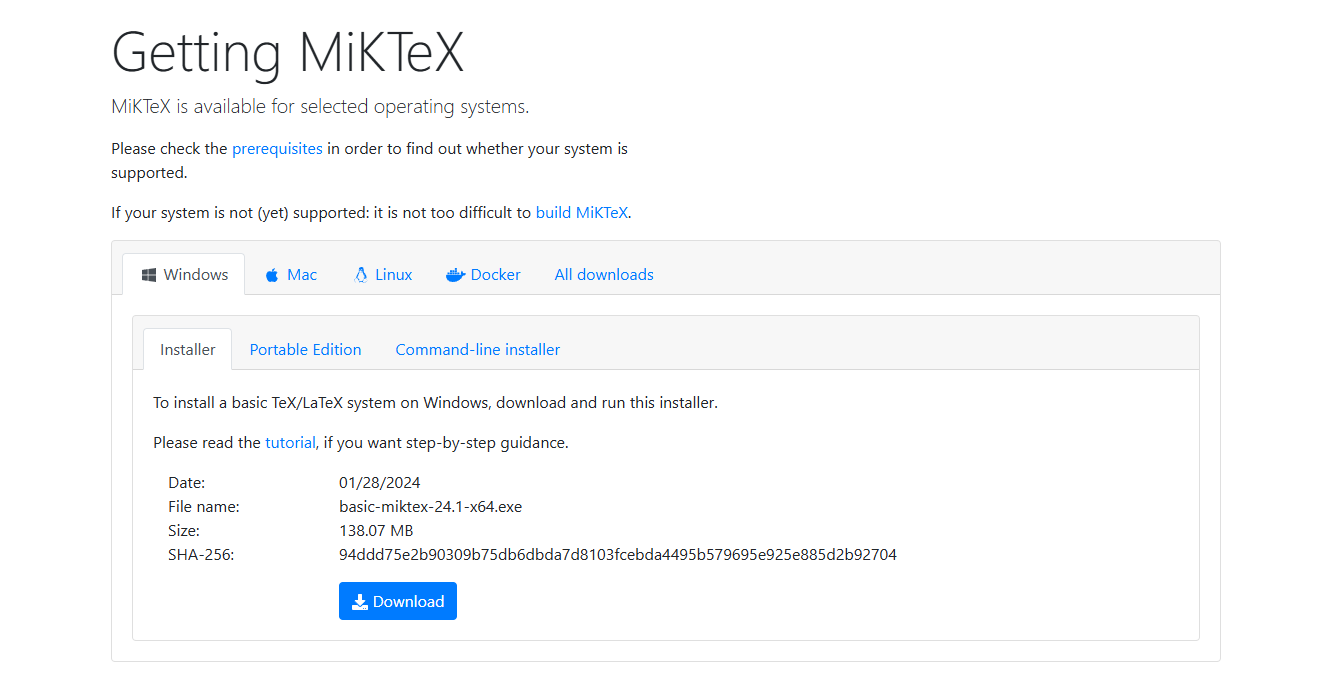
\includegraphics[width=\textwidth, height=0.5\textheight, keepaspectratio]{mike.png}
\end{figure}

\begin{enumerate}
    \setcounter{enumi}{2} 
    \item Ejecuta el instalador y sigue los pasos: siguiente → siguiente → terminar.
    
   
    \begin{figure}[h!]
        \centering
        
\includegraphics[width=\textwidth, height=0.5\textheight, keepaspectratio]{instalador mike.png}
    \end{figure}

    \item Una vez instalado, abre \textbf{TeXworks} (incluido con MiKTeX) para probarlo.
\end{enumerate}


\section{Instalación de Strawberry Perl}
Algunos paquetes de LaTeX requieren Perl (ej: \texttt{latexmk}).  

\begin{enumerate}
    \item Descarga \textbf{Strawberry Perl} desde 
    \href{http://strawberryperl.com/}{strawberryperl.com}.
    
    % Imagen justo después del primer ítem
    \begin{flushleft}
    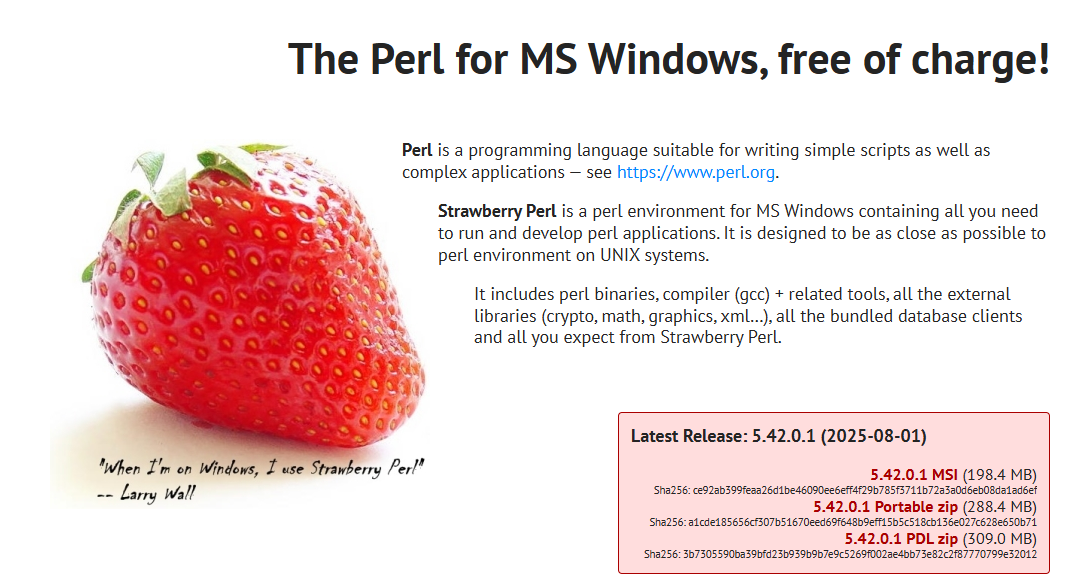
\includegraphics[width=0.7\textwidth, keepaspectratio]{straw.png}
    \end{flushleft}

    

    \item Ejecuta el instalador y sigue los pasos por defecto.
    
\end{enumerate}



\section{Creación de carpeta de trabajo}


\begin{enumerate}
    \item Crea una carpeta en tu PC donde guardarás todos tus archivos `.tex`, por ejemplo: \texttt{C:\textbackslash MisDocumentosLaTeX}.
    \item Coloca tus imágenes y recursos dentro de esa carpeta para que LaTeX los pueda localizar fácilmente.
\end{enumerate}

\section{Prueba de compilación}
\begin{enumerate}
    \item Abre tu editor (TeXworks, TeXstudio, VSCode con LaTeX Workshop, etc.).
    \item Escribe el siguiente código en un archivo nuevo llamado \texttt{prueba.tex}:
\end{enumerate}

\begin{lstlisting}
\documentclass{article}
\begin{document}

\end{document}
\end{lstlisting}

\begin{enumerate}
    \item Haz clic en \textbf{Compilar} (pdflatex).
    \item Se generará un PDF con el texto ``¡Hola, LaTeX!'' 
\end{enumerate}

\section{Consejos adicionales}
\begin{itemize}
    \item No uses latex, usa google docs u otra cosa.
   
\end{itemize}

\end{document}
